
\OPGAVE
{
\section{Generaliseerbaarheidstheorie - Voorbeeld 1}

Het practicum ontwikkelingspsychologie II bestaat uit een schriftelijk verslag met 10 vragen dat elke student dient in te vullen. De antwoorden op de vragen worden door twee beoordelaars ge\"{e}valueerd waarbij elke beoordelaar alle 10 de vragen scoort.\\
Na toepassing van een variantie-analyse wordt de volgende schatting van de variantiecomponenten bekomen:

\begin{center}
\renewcommand{\arraystretch}{1.2}
\begin{tabular}{|c|c|c|c|c|c|c|c|} \hline
 & $ \hat{\sigma}^2_{s} $ & $ \hat{\sigma}^2_{v} $& $ \hat{\sigma}^2_{b} $ & $ \hat{\sigma}^2_{sv} $ & $ \hat{\sigma}^2_{sb} $ & $ \hat{\sigma}^2_{vb} $ & $ \hat{\sigma}^2_{svb,e} $ \\ \hline
Waarde  & $ 0.397 $ & $ 0.109 $ & $ 0.010 $ & $ 0.314 $ & $ 0.067 $ & $ 0.006 $ & $ 0.224 $ \\
\% Var & $ 35 $ & $ 10 $ & $ 1 $ & $ 28 $ & $ 6 $ & $ 1 $ & $ 20 $ \\ \hline
\end{tabular}
\end{center}


\normalsize
De gegevens uit de tabel kunnen gebruikt worden om volgende vragen te beantwoorden.

\begin{enumerate}
\item JUIST of FOUT: ``Idealiter is $ \hat{\sigma}^2_{s} $ substantieel groter dan $ \hat{\sigma}^2_{v}$"?
\item Stel, de verantwoordelijke lesgever zou graag in volgende jaren de werklast voor de beoordelaars opsplitsen (situatie 2).
Beoordelaar 1 zou dan enkel vraag 1-5 verbeteren, terwijl beoordelaar 2 vraag 6-10 zou verbeteren.
Hoe ziet ons model eruit, gebruik makende van de symbolen $s$, $v$ en $b$?
\item Bereken de generaliseerbaarheidsco\"{e}ffici\"{e}nt (G) voor deze nieuwe situatie (2).

\item Stel, de verantwoordelijke lesgever vraagt zich af of wel alle 10 de vragen noodzakelijk zijn. Bepaal met behulp van een $D$-studie de hoeveelheid vragen die minimaal nodig is (gebruik makend van 2 beoordelaars) om toch een meetnauwkeurigheid van 0.85 te behouden.

\end{enumerate}
}

\OPLOSSING
{
\textbf{Oplossingen}
\begin{enumerate}
\item JUIST. Dit impliceert dat het grootste deel van de bekomen variantie subjectgerelateerd is, eerder dan aan meetfacetten gerelateerd.
\item $s \times v(b)$
\begin{center}
\begin{figure}[H]
\begin{adjustwidth}{}{-0in}
\begin{center}
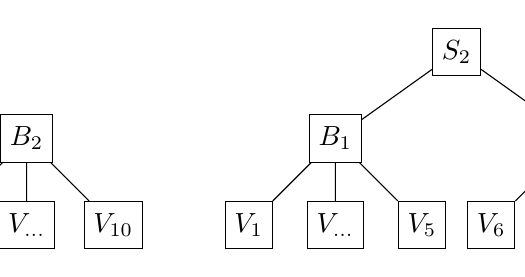
\begin{tikzpicture}[
scale=0.55,
level distance=20mm,
level 1/.style={sibling distance=56mm},
level 2/.style={sibling distance=20mm},
level 3/.style={sibling distance=12mm},
level 4/.style={sibling distance=12mm}
]

\usetikzlibrary{shapes}
\tikzstyle{c} = [draw, shape=rectangle, minimum size = 6mm]
\tikzstyle{r} = [draw, shape=rectangle,minimum width=10mm]
\tikzstyle{tr} = [draw,isosceles triangle, shape border rotate=90, anchor=north]

\hspace*{-4.5 cm}

\node[c] {$S_{1}$}
child{node[c]{$B_{1}$}
	child{node[c]{$V_{1}$}}
	child{node[c]{$V_{\ldots}$}}
	child{node[c]{$V_{5}$}}
	}
child{node[c]{$B_{2}$}
	child{node[c]{$V_{6}$}}
	child{node[c]{$V_{\ldots}$}}
	child{node[c]{$V_{10}$}}
	}
;\hspace*{7 cm}
\node[c] {$S_{2}$}
child{node[c]{$B_{1}$}
	child{node[c]{$V_{1}$}}
	child{node[c]{$V_{\ldots}$}}
	child{node[c]{$V_{5}$}}
	}
child{node[c]{$B_{2}$}
	child{node[c]{$V_{6}$}}
	child{node[c]{$V_{\ldots}$}}
	child{node[c]{$V_{10}$}}
	}
;\hspace*{4.5 cm}
\node[c] {$S_{...}$}
child{node[c]{{...}}
	child{node[c]{$\ldots$}}
	}
	;
	
\end{tikzpicture}
\caption{S = subjecten, B = beoordelaars en V = vragen. ``$\ldots$" = alle overige waarden analoog aan $S_1$ en $S_{2}$. }\label{f.gen1}
\end{center}
\end{adjustwidth}
\end{figure}

\end{center}
\newpage
\item De G-co\"{e}ffici\"{e}nt wordt als volgt berekend:\\
	% G-coefficient
	\begin{align}
		G &=\dfrac{\sigma^2_{Obj~v.~met.}}{\sigma^2_{Obj~v.~met.}+ \sigma^2_{rel.~meting}} \label{eq.G1}
	\end{align}
	Merk op dat we hier te maken hebben met de volgende niet te onderscheiden variantiecomponenten:~ \\
	$ \bm{\hat{\sigma}^2_{v}} $~en~$\bm{\hat{\sigma}^2_{vb} }$.\\
	We kunnen dus enkel gebruik maken van de volgende gegevens: \\
	\begin{tabular}{|c|c|c|c|c|c|c|c|} \hline
	 & $ \hat{\sigma}^2_{s}$ & $ \hat{\sigma}^2_{b} $& $ \hat{\sigma}^2_{v,vb} $ & $ \hat{\sigma}^2_{sb}$ & $\hat{\sigma}^2_{sv} $ & $ \hat{\sigma}^2_{vb} $& $ \hat{\sigma}^2_{sv, svb, e} $ \\ \hline
	$\sigma^2 $  			& $ 0.397 $ 			& $ 0.010 $ 			& $0.109+0.006  $ 			& $ 0.067 $				 & $. $	& $ . $& $ 0.314 + 0.224  $ \\
	$n_.$				& .						& 2					& 20				 		& 2			  		 & $. $	& $ . $&  20 \\ \hline
	$\sigma^2 / n$ 		& .						& 0.005				& 0.00575				 		& 0.0335			  	 & $. $	& $ . $&  0.269 \\ \hline
	\end{tabular} \\

  We berekenen hiervoor eerst $\sigma^2_{rel.~meting}$
  \begin{align*}
    \sigma^2_{rel.~meting} 	&=  \dfrac{\hat{\sigma}^2_{sb}}{n_b} + \dfrac{\hat{\sigma}^2_{sv,svb,e}}{n_v*n_b} \\
                &=  \dfrac{{0.067}}{2} + \dfrac{{0.314 + 0.224}}{10*2}\\
                &= 0.0335 + 0.0269 \\
                &= 0.0604
  \end{align*}
  Bijgevolg kan $G$ opgesteld worden door $\sigma^2_{rel.~meting}$ en $\hat{\sigma}^2_{s}$ in te vullen in vergelijking \ref{eq.G1}:
  \begin{align*}
    G 	&=\dfrac{0.397}{0.397 + 0.0604}\\
      &=0.87
  \end{align*}
\item We berekenen voor de vector \textbf{v} = \{9,8,7,6,5,4,3,2,1\}, aantal vragen die aangeboden worden, telkens de G-co\"{e}ffici\"{e}nt. Deze is gelijk aan:

\begin{center}
\renewcommand{\arraystretch}{1.2}
\hspace*{-3 cm}
\begin{tabular}{|l|c|c|c|c|c|c|c|c|c|} \hline
 \textbf{v} & $ 9 $ & $ 8 $& $ 7 $ & $ 6 $ & $ 5 $ & $ 4 $ & $ 3 $ & $ 2 $ & $ 1 $ \\ \hline
G  & 0.$8623145$ & $0.855373$ & $0.8466108$ & $0.8352034$ & $0.8197398$ & $0.7975892$ & $0.7632169$ & $0.7026549$ & $0.5675482$ \\ \hline
\end{tabular}
\end{center}
We besluiten dus dat 8 vragen voldoende zijn om een meetnauwkeurigheid van 0.85 te behalen.
\end{enumerate}
}

\newpage

\OPGAVE
{
\section{Generaliseerbaarheidstheorie - Voorbeeld 2}

Een verkorte vorm van de TAT (Thematic Apperception Test), bestaande uit 10 kaarten, wordt afgenomen bij 50
jongvolwassen delinquenten ($d$).
De TAT is zo opgesteld dat de juveniele delinquent bij elk van de 10 kaarten ($k$) een verhaal moet vertellen dat aansluit bij de tekening op de kaart.
De tien verhalen werden op video opgenomen en later beoordeeld.
3 klinische psychologen ($p$) beoordeelden elk de graad van \emph{rejection of authority} op een schaal van 0 tot 100.
De finale score op de TAT is het gemiddelde van de 30 metingen per subject. \footnote{
Naar Hoofdstuk 8 oef 3.a uit Crocker and Algina (2008). \emph{Introduction to Classical and Modern Test Theory}.}

\begin{center}
\renewcommand{\arraystretch}{1.2}
\begin{tabular}{|c|c|c|c|c|c|c|c|} \hline
 & $ \hat{\sigma}^2_{d} $ & $ \hat{\sigma}^2_{k} $& $ \hat{\sigma}^2_{p} $ & $ \hat{\sigma}^2_{dk} $ & $ \hat{\sigma}^2_{dp} $ & $ \hat{\sigma}^2_{kp} $ & $ \hat{\sigma}^2_{dkp,e} $ \\ \hline
Waarde  & $ 167.64 $ & $ 3.211 $ & $615.8 $ & $ 1.3 $ & $ 84.7 $ & $ 1.3 $ & $ 1.2 $ \\
\% Var & 0.1923& 0.004& 0.704& 0.001& 0.097& 0.001& 0.001 \\ \hline
\end{tabular}
\end{center}

\normalsize
De gegevens uit de tabel kunnen gebruikt worden om volgende vragen te beantwoorden.

\begin{enumerate}
	\item Schrijf deze opstelling uit.
	\item JUIST of FOUT: ``In deze opstelling kunnen er meer variantie-componenten worden onderscheiden dan wanneer elke $p$ een beperkte (unieke) set van vragen toebedeeld krijgt."?
	\item \emph{tip: schrijf bij deze vraag telkens eerst het opzet uit}\\
	Welke variantie-componenten kunnen niet meer van elkaar onderscheiden worden indien voor een geplande $D$-studie met evenveel delinquenten volgende opzetten gehanteerd worden:
\begin{itemize}
	\item $p_1$ beoordeelt vragen 1 en 4, $p_2$ vragen 5 en 8 en $p_3$ vragen 9 en 10?
	\item De zware delinquenten in kwestie  zitten verspreid over 50 instellingen (1 per instelling) waarbij er per instelling slechts twee psychologen beschikbaar zijn (telkens twee andere psychologen). 
	Per instelling behandelen deze twee psychologen altijd dezelfde drie kaarten: 1,2 en 3. 
\end{itemize}
\item Bereken voor het eerste scenario uit 3 de $G$-co\"{e}ffici\"{e}nt en voor het tweede scenario de index of dependability $\phi$. Waar ligt het verschil tussen beide maten?
\end{enumerate}
}

\OPLOSSING
{
\textbf{Oplossingen}
\begin{enumerate}
\item $d \times p \times k$
\begin{figure}[H]
\begin{adjustwidth}{}{-0in}
\begin{center}
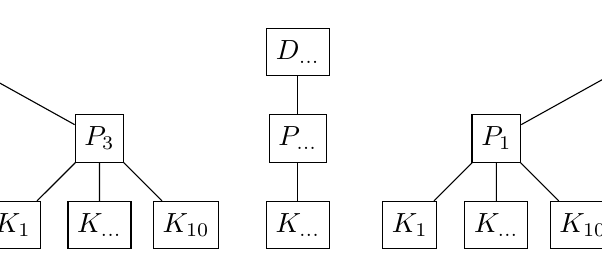
\begin{tikzpicture}[
scale=0.55,
level distance=20mm,
level 1/.style={sibling distance=36mm},
level 2/.style={sibling distance=20mm},
level 3/.style={sibling distance=12mm},
level 4/.style={sibling distance=12mm}
]

\usetikzlibrary{shapes}
\tikzstyle{c} = [draw, shape=rectangle, minimum size = 6mm]
\tikzstyle{r} = [draw, shape=rectangle,minimum width=10mm]
\tikzstyle{tr} = [draw,isosceles triangle, shape border rotate=90, anchor=north]

\hspace*{-4.5 cm}

\node[c] {$D_{1}$}
child{node[c]{$P_{1}$}
	child{node[c]{$K_{1}$}}
	child{node[c]{$K_{\ldots}$}}
	child{node[c]{$K_{10}$}}
	}
child{node[c]{$P_{2}$}
	child{node[c]{$K_{\ldots}$}}
	}
child{node[c]{$P_{3}$}
	child{node[c]{$K_{1}$}}
	child{node[c]{$K_{\ldots}$}}
	child{node[c]{$K_{10}$}}
	}
;\hspace*{4.5 cm}
\node[c] {$D_{...}$}
child{node[c]{$P_{...}$}
	child{node[c]{$K_{\ldots}$}}
	}
;\hspace*{4.5 cm}
\node[c] {$D_{50}$}
child{node[c]{$P_{1}$}
	child{node[c]{$K_{1}$}}
	child{node[c]{$K_{\ldots}$}}
	child{node[c]{$K_{10}$}}
	}
child{node[c]{$P_{2}$}
	child{node[c]{$K_{\ldots}$}}
	}
child{node[c]{$P_{3}$}
	child{node[c]{$K_{1}$}}
	child{node[c]{$K_{\ldots}$}}
	child{node[c]{$K_{10}$}}
	}
;

\end{tikzpicture}
\caption{D = delinquent, P = psycholoog en K = kaart. ``$\ldots$" = alle overige waarden. }\label{f.gen}
\end{center}
\end{adjustwidth}
\end{figure}

\item JUIST. In een volledig gekruist opzet kunnen steeds meer variantiecomponenten onderscheiden worden dan in om het even welk genest opzet dat gebruik maakt van dezelfde meetfacetten. 
\item
\begin{itemize}
	\item Het opzet wordt hier: $d \times k\left(p\right)$ bijgevolg kunnen de variantiecomponenten $\hat{\sigma}^2_p$ en $\hat{\sigma}^2_{kp}$ niet onderscheiden worden van elkaar (wordt $\hat{\sigma}^2_{pk,p}$) en ook $\hat{\sigma}^2_{dk}$ kan niet van de residuele variantie-term worden onderscheiden (wordt $\hat{\sigma}^2_{dk, dpk,e}$). Dit zijn de te onderscheiden componenten:\\ Merk hierbij op dat het object van meting $d$ is. \\
	\begin{tabular}{|c|c|c|c|c|c|c|c|} \hline
	 & $ \hat{\sigma}^2_{d}$ & $ \hat{\sigma}^2_{k} $& $ \hat{\sigma}^2_{p,kp} $ & $ \hat{\sigma}^2_{dk}$ & $\hat{\sigma}^2_{kp} $ & $ \hat{\sigma}^2_{dp} $& $ \hat{\sigma}^2_{dk, dkp, e} $ \\ \hline
	$\sigma^2$  			& $ 167.64 $ 			& $ 3.211 $ 			& $615.8+1.3  $ 			& $ .$				 & $. $	& $ 84.7 $	 & $ 1.2 + 1.3  $ \\
	$n_.$				& .						& 6						& 3*6				 		& $ .$		  		 & $. $	& $ 3 $		 &  3*6 \\ \hline
	$\sigma^2 / n$ 		& .						& 0.5352				& 34.2833				 	& $ .$			  	 & $. $	& $ 28.2333 $& 0.1389 \\ \hline
	\end{tabular} \\
	De grafische weergave van dit opzet is het volgende:\\
	\begin{figure}[H]
\begin{adjustwidth}{}{-0in}
\begin{center}
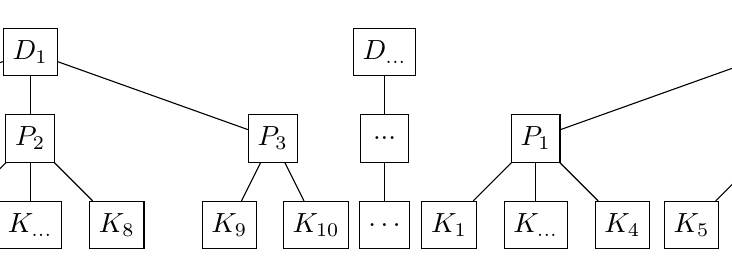
\begin{tikzpicture}[
scale=0.55,
level distance=20mm,
level 1/.style={sibling distance=56mm},
level 2/.style={sibling distance=20mm},
level 3/.style={sibling distance=12mm},
level 4/.style={sibling distance=12mm}
]

\usetikzlibrary{shapes}
\tikzstyle{c} = [draw, shape=rectangle, minimum size = 6mm]
\tikzstyle{r} = [draw, shape=rectangle,minimum width=10mm]
\tikzstyle{tr} = [draw,isosceles triangle, shape border rotate=90, anchor=north]

\hspace*{-4.5 cm}

\node[c] {$D_{1}$}
child{node[c]{$P_{1}$}
	child{node[c]{$K_{1}$}}
	child{node[c]{$K_{\ldots}$}}
	child{node[c]{$K_{4}$}}
	}
child{node[c]{$P_{2}$}
	child{node[c]{$K_{5}$}}
	child{node[c]{$K_{\ldots}$}}
	child{node[c]{$K_{8}$}}
	}
child{node[c]{$P_{3}$}
	child{node[c]{$K_{9}$}}
	child{node[c]{$K_{10}$}}
	}
;\hspace*{4.5 cm}
\node[c] {$D_{...}$}
child{node[c]{{...}}
	child{node[c]{$\ldots$}}
	}
;\hspace*{5 cm}
\node[c] {$D_{50}$}
child{node[c]{$P_{1}$}
	child{node[c]{$K_{1}$}}
	child{node[c]{$K_{\ldots}$}}
	child{node[c]{$K_{4}$}}
	}
child{node[c]{$P_{2}$}
	child{node[c]{$K_{5}$}}
	child{node[c]{$K_{\ldots}$}}
	child{node[c]{$K_{8}$}}
	}
child{node[c]{$P_{3}$}
	child{node[c]{$K_{9}$}}
	child{node[c]{$K_{10}$}}
	};
\end{tikzpicture}
\caption{D = delinquent, P = psycholoog en K = kaart. ``$\ldots$" = alle overige waarden analoog aan $D_1$ en $D_{50}$. }\label{f.gen2A}
\end{center}
\end{adjustwidth}
\end{figure}

	
	\item Het opzet wordt hier: $p\left(k\times d\right)$. Bijgevolg kunnen de variantiecomponenten $\hat{\sigma}^2_p$, $\hat{\sigma}^2_{kp}$ en $\hat{\sigma}^2_{pd}$ niet onderscheiden worden van de residuele variantie-term onderscheiden (wordt $\hat{\sigma}^2_{p, kp, pd, dpk, e}$). Houd rekening met het verminderde aantal kaarten ($K$).\\Dit zijn de te onderscheiden componenten:\\ Merk hierbij opnieuw op dat het object van meting $d$ is. \\

	\begin{tabular}{|c|c|c|c|c|c|c|c|} \hline
	 & $ \hat{\sigma}^2_{d} $ & $ \hat{\sigma}^2_{k} $& $ \hat{\sigma}^2_{p} $ & $ \hat{\sigma}^2_{dk} $ & $ \hat{\sigma}^2_{dp} $ & $ \hat{\sigma}^2_{kp} $ &
	 $\hat{\sigma}^2_{p, kp, dp, dpk, e}$ \\ \hline
	$\sigma^2$  			& $167.64$ 			& $ 3.211 $  	& . 	  & $1.3$				 & $ . $	& $ . $& $ 1.2 + 1.3 +  615.8 +84.7$ \\
	$n_.$ 				& . 					& $3$			& .	  & $ 3$		  		 & $ . $ 	& $ . $&  $2 *3$ \\ \hline
	$\sigma^2 / n_.$      & .						& $1.0703 $		& .   & $0.4333$			  	 & $.$	& $ . $&  103.2667 \\ \hline
	\end{tabular} \\
	De grafische weergave van dit opzet is het volgende:\\

	\begin{figure}[H]
\begin{adjustwidth}{}{-0in}
\begin{center}
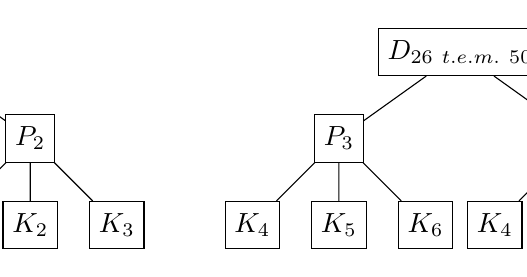
\begin{tikzpicture}[
scale=0.55,
level distance=20mm,
level 1/.style={sibling distance=56mm},
level 2/.style={sibling distance=20mm},
level 3/.style={sibling distance=12mm},
level 4/.style={sibling distance=12mm}
]

\usetikzlibrary{shapes}
\tikzstyle{c} = [draw, shape=rectangle, minimum size = 6mm]
\tikzstyle{r} = [draw, shape=rectangle,minimum width=10mm]
\tikzstyle{tr} = [draw,isosceles triangle, shape border rotate=90, anchor=north]

\hspace*{-4.5 cm}

\node[c] {$D_{1~t.e.m.~25}$}
child{node[c]{$P_{1}$}
	child{node[c]{$K_{1}$}}
	child{node[c]{$K_{2}$}}
	child{node[c]{$K_{3}$}}
	}
child{node[c]{$P_{2}$}
	child{node[c]{$K_{1}$}}
	child{node[c]{$K_{2}$}}
	child{node[c]{$K_{3}$}}
	}
;\hspace*{7 cm}
\node[c] {$D_{26~t.e.m.~50}$}
child{node[c]{$P_{3}$}
	child{node[c]{$K_{4}$}}
	child{node[c]{$K_{5}$}}
	child{node[c]{$K_{6}$}}
	}
child{node[c]{$P_{4}$}
	child{node[c]{$K_{4}$}}
	child{node[c]{$K_{5}$}}
	child{node[c]{$K_{6}$}}
	}
;
\end{tikzpicture}
\caption{D = delinquent, P = psycholoog en K = kaart. }\label{f.gen2B}
\end{center}
\end{adjustwidth}
\end{figure}

\end{itemize}
%v <- c(167.64,3.211,615.8,1.3,84.7,1.3,1.2)
%np =3
%nk =10

\item Respectievelijk de $G$ en $\phi$ co\"effici\"ent:
\begin{itemize}
	% G-coefficient
	\item	Houd rekening met volgende niet te onderscheiden variantiecomponenten:~ 
	$ \bm{\hat{\sigma}^2_{p,kp}} $~en~$\bm{\hat{\sigma}^2_{dk, dkp, e} }$.\\
	We berekenen hiervoor eerst $\sigma^2_{rel.~meting}$
	\begin{align*}
		\sigma^2_{rel.~meting} 	&=  \dfrac{\hat{\sigma}^2_{dp}}{n_k} + \dfrac{\hat{\sigma}^2_{dk,dpk,e}}{n_p*n_k} \\
								&=  \dfrac{{84.7}}{3} + \dfrac{{1.2 + 1.3}}{3*6}\\
								&= 28.2333 + 0.1389 &= 28.3722
	\end{align*}
	Bijgevolg kan $G$ opgesteld worden door $\sigma^2_{rel.~meting}$ en $\hat{\sigma}^2_{d}$ in te vullen in vergelijking \ref{eq.G1}:
	\begin{align*}
		G 	&=\dfrac{167.64}{167.64+  28.3722}\\
			&=\dfrac{167.64}{ 196.0122}&=0.8553
	\end{align*}

	% PHI-coefficient
	\item
	\begin{align}
		\phi =\dfrac{\sigma^2_{Obj~v.~met.}}{\sigma^2_{Obj~v.~met.}+ \sigma^2_{abs.~meting}} \label{eq.phi}
	\end{align}
	Houd voorts rekening met volgende niet te onderscheiden variantiecomponenten:~ \\
	$\bm{\hat{\sigma}^2_p},\bm{\hat{\sigma}^2_{dp}} , \bm{\hat{\sigma}^2_{kp}} \text{ en } \bm{\hat{\sigma}^2_{dkp, e}}$.\\
	We berekenen hiervoor eerst $\sigma^2_{abs.~meting}$
	\begin{align*}
		\sigma^2_{abs.~meting} 	&=  \dfrac{\hat{\sigma}^2_{k}}{n_k} + \dfrac{\hat{\sigma}^2_{p, kp, dp, dpk, e}}{n_p*n_k} \\
								&=  \dfrac{{3.122}}{3} + \dfrac{{1.2 + 1.3 +  615.8 +84.7}}{2*3}\\
								&=  1.0703 + 117.1667 &= 118.237
	\end{align*}
	Bijgevolg kan $\phi$ opgesteld worden door $\sigma^2_{abs. meting}$ en $\hat{\sigma}^2_{d}$ in te vullen in vergelijking \ref{eq.phi}:
	\begin{align*}
		\phi 	&=\dfrac{167.64}{167.64+  118.237}\\
				&=\dfrac{167.64}{285.877}=0.5864
	\end{align*}
	\end{itemize}
	\item \begin{description}
		\item[$G$] Door gebruik te maken van de relatieven metingen wordt de prestatie uitgedrukt in relatieve termen, t.t.z. de variantiecomponententen hebben telkens betrekking op zowel de meetfacetten als het object van meting. 
		\item[$\phi$] Door gebruik te maken van de absolute metingen wordt de meetnauwkeurigheid van een meetprocedure uitgedrukt door deze co\"efficient.
		Dit heeft betrekking tot de bepaling van de \emph{universum}score.
	\end{description}
	
\end{enumerate}
}
